\documentclass{beamer}

\usepackage[T1]{fontenc}
\usepackage{lmodern}
\usepackage{graphicx}
\usepackage{amsmath}
\usepackage{amssymb}
\usepackage{booktabs}
\usepackage{xcolor}
\usepackage{tikz}
\usepackage{array}
\usepackage{colortbl}
\usepackage[authoryear,round]{natbib}
\usepackage{ragged2e}

\usetheme{Madrid}
\usecolortheme{default}
\setbeamertemplate{navigation symbols}{}
\setbeamertemplate{footline}[frame number]
\setbeamersize{text margin left=0.6cm, text margin right=0.6cm}

\definecolor{myprimary}{HTML}{FF9D00}
\definecolor{mysecondary}{HTML}{FF8360}
\definecolor{mydark}{HTML}{243447}
\definecolor{mylight}{HTML}{FFF4E8}
\definecolor{mysoft}{HTML}{F7F7F7}

\setbeamercolor{structure}{fg=myprimary}
\setbeamercolor{title}{fg=white,bg=myprimary}
\setbeamercolor{subtitle}{fg=myprimary}
\setbeamercolor{frametitle}{fg=white,bg=myprimary!90}
\setbeamercolor{block title}{fg=white,bg=myprimary!85}
\setbeamercolor{block body}{fg=black,bg=mylight}
\setbeamercolor{normal text}{fg=mydark,bg=white}
\setbeamercolor{alerted text}{fg=mysecondary}

\setbeamerfont{title}{series=\bfseries,size=\Large}
\setbeamerfont{frametitle}{series=\bfseries,size=\large}
\setbeamerfont{block title}{series=\bfseries}
\setbeamertemplate{bibliography item}[text]
\setlength{\bibsep}{1pt plus 0.2ex}
\bibliographystyle{abbrvnat}

\newcommand{\lerobot}{\texttt{lerobot}}
\newcommand{\lerobotdataset}{\texttt{LeRobotDataset}}
\newcommand{\pizero}{\(\pi_0\)}
\newcommand{\highlight}[1]{\textcolor{myprimary}{\textbf{#1}}}
\newcommand{\statbox}[2]{%
  \begingroup
  \setlength{\fboxsep}{8pt}%
  \colorbox{mylight}{\parbox{\dimexpr\linewidth-2\fboxsep\relax}{\raggedright\textbf{\large #1}\\[-1pt]\small #2}}%
  \endgroup
}

\newcommand{\circled}[1]{%
  \tikz[baseline=(char.base)]\node[draw,circle,inner sep=1pt,thick](char){\textbf{#1}};%
}

\newcommand{\lightbox}[1]{%
  \tikz[baseline=(txt.base)]{
    \node[
      fill=myprimary!15,
      rounded corners=2pt,
      inner xsep=4pt,
      inner ysep=1.5pt
    ] (txt) {\strut #1};
  }%
}

\newcommand{\commonauthors}{%
  Francesco Capuano \and
  Caroline Pascal \and
  Adil Zouitine \and
  Thomas Wolf \and
  Michel Aractingi
}

\newcommand{\shortauthors}{%
  Francesco Capuano, Caroline Pascal, Adil Zouitine, Thomas Wolf, Michel Aractingi
}

\newcommand{\chaptertitleframe}[1]{%
  \begin{frame}[plain]
    \vspace{0.35cm}
    \begin{center}
      \begin{beamercolorbox}[wd=0.86\paperwidth,rounded=true,sep=10pt,center]{title}
        \usebeamerfont{title}\inserttitle
      \end{beamercolorbox}

      \vspace{0.55cm}
      {\Large\bfseries\textcolor{myprimary}{\insertsubtitle}\par}
      \vspace{0.15cm}
      {\small\color{mydark}\shortauthors\par}

      \vspace{0.45cm}
      
\includegraphics[height=1.0cm]{hf.pdf}
      \hspace{0.45cm}
      
\includegraphics[height=0.95cm]{oxford_logo.png}

      \vspace{0.55cm}
      \begin{beamercolorbox}[wd=0.8\paperwidth,rounded=true,sep=8pt,center]{block body}
        \small #1
      \end{beamercolorbox}
    \end{center}
  \end{frame}
}

\newcommand{\sources}[1]{%
  \vfill
  {\raggedright\tiny\color{black!65}\textbf{Refs:} #1\par}
}

\graphicspath{{../../../figures/}{../../../logos/}}

\title[Robot Learning Tutorial]{Robot Learning: A Tutorial}
\subtitle{Chapter 3: Robot Reinforcement Learning}
\author[Capuano et al.]{\commonauthors}
\date{}
\titlegraphic{
  \vspace{-1.1cm}
  
\includegraphics[height=1.4cm]{hf.pdf}
  \hspace{0.3cm}
  
\includegraphics[height=1.2cm]{oxford_logo.png}
}

\begin{document}

\chaptertitleframe{Why RL is a natural fit for robotics, why naive real-world RL fails, and how data-driven real-world pipelines make it usable.}

\begin{frame}{Roadmap}
  \begin{enumerate}
    \item Why RL is appealing in robotics
    \item The RL loop and its core objects
    \item Why real-world RL is hard
    \item How sample-efficient real-world pipelines like HIL-SERL help
  \end{enumerate}
\end{frame}

\begin{frame}{Why RL Enters Robotics}
  \begin{columns}[T,onlytextwidth]
    \begin{column}{0.54\textwidth}
      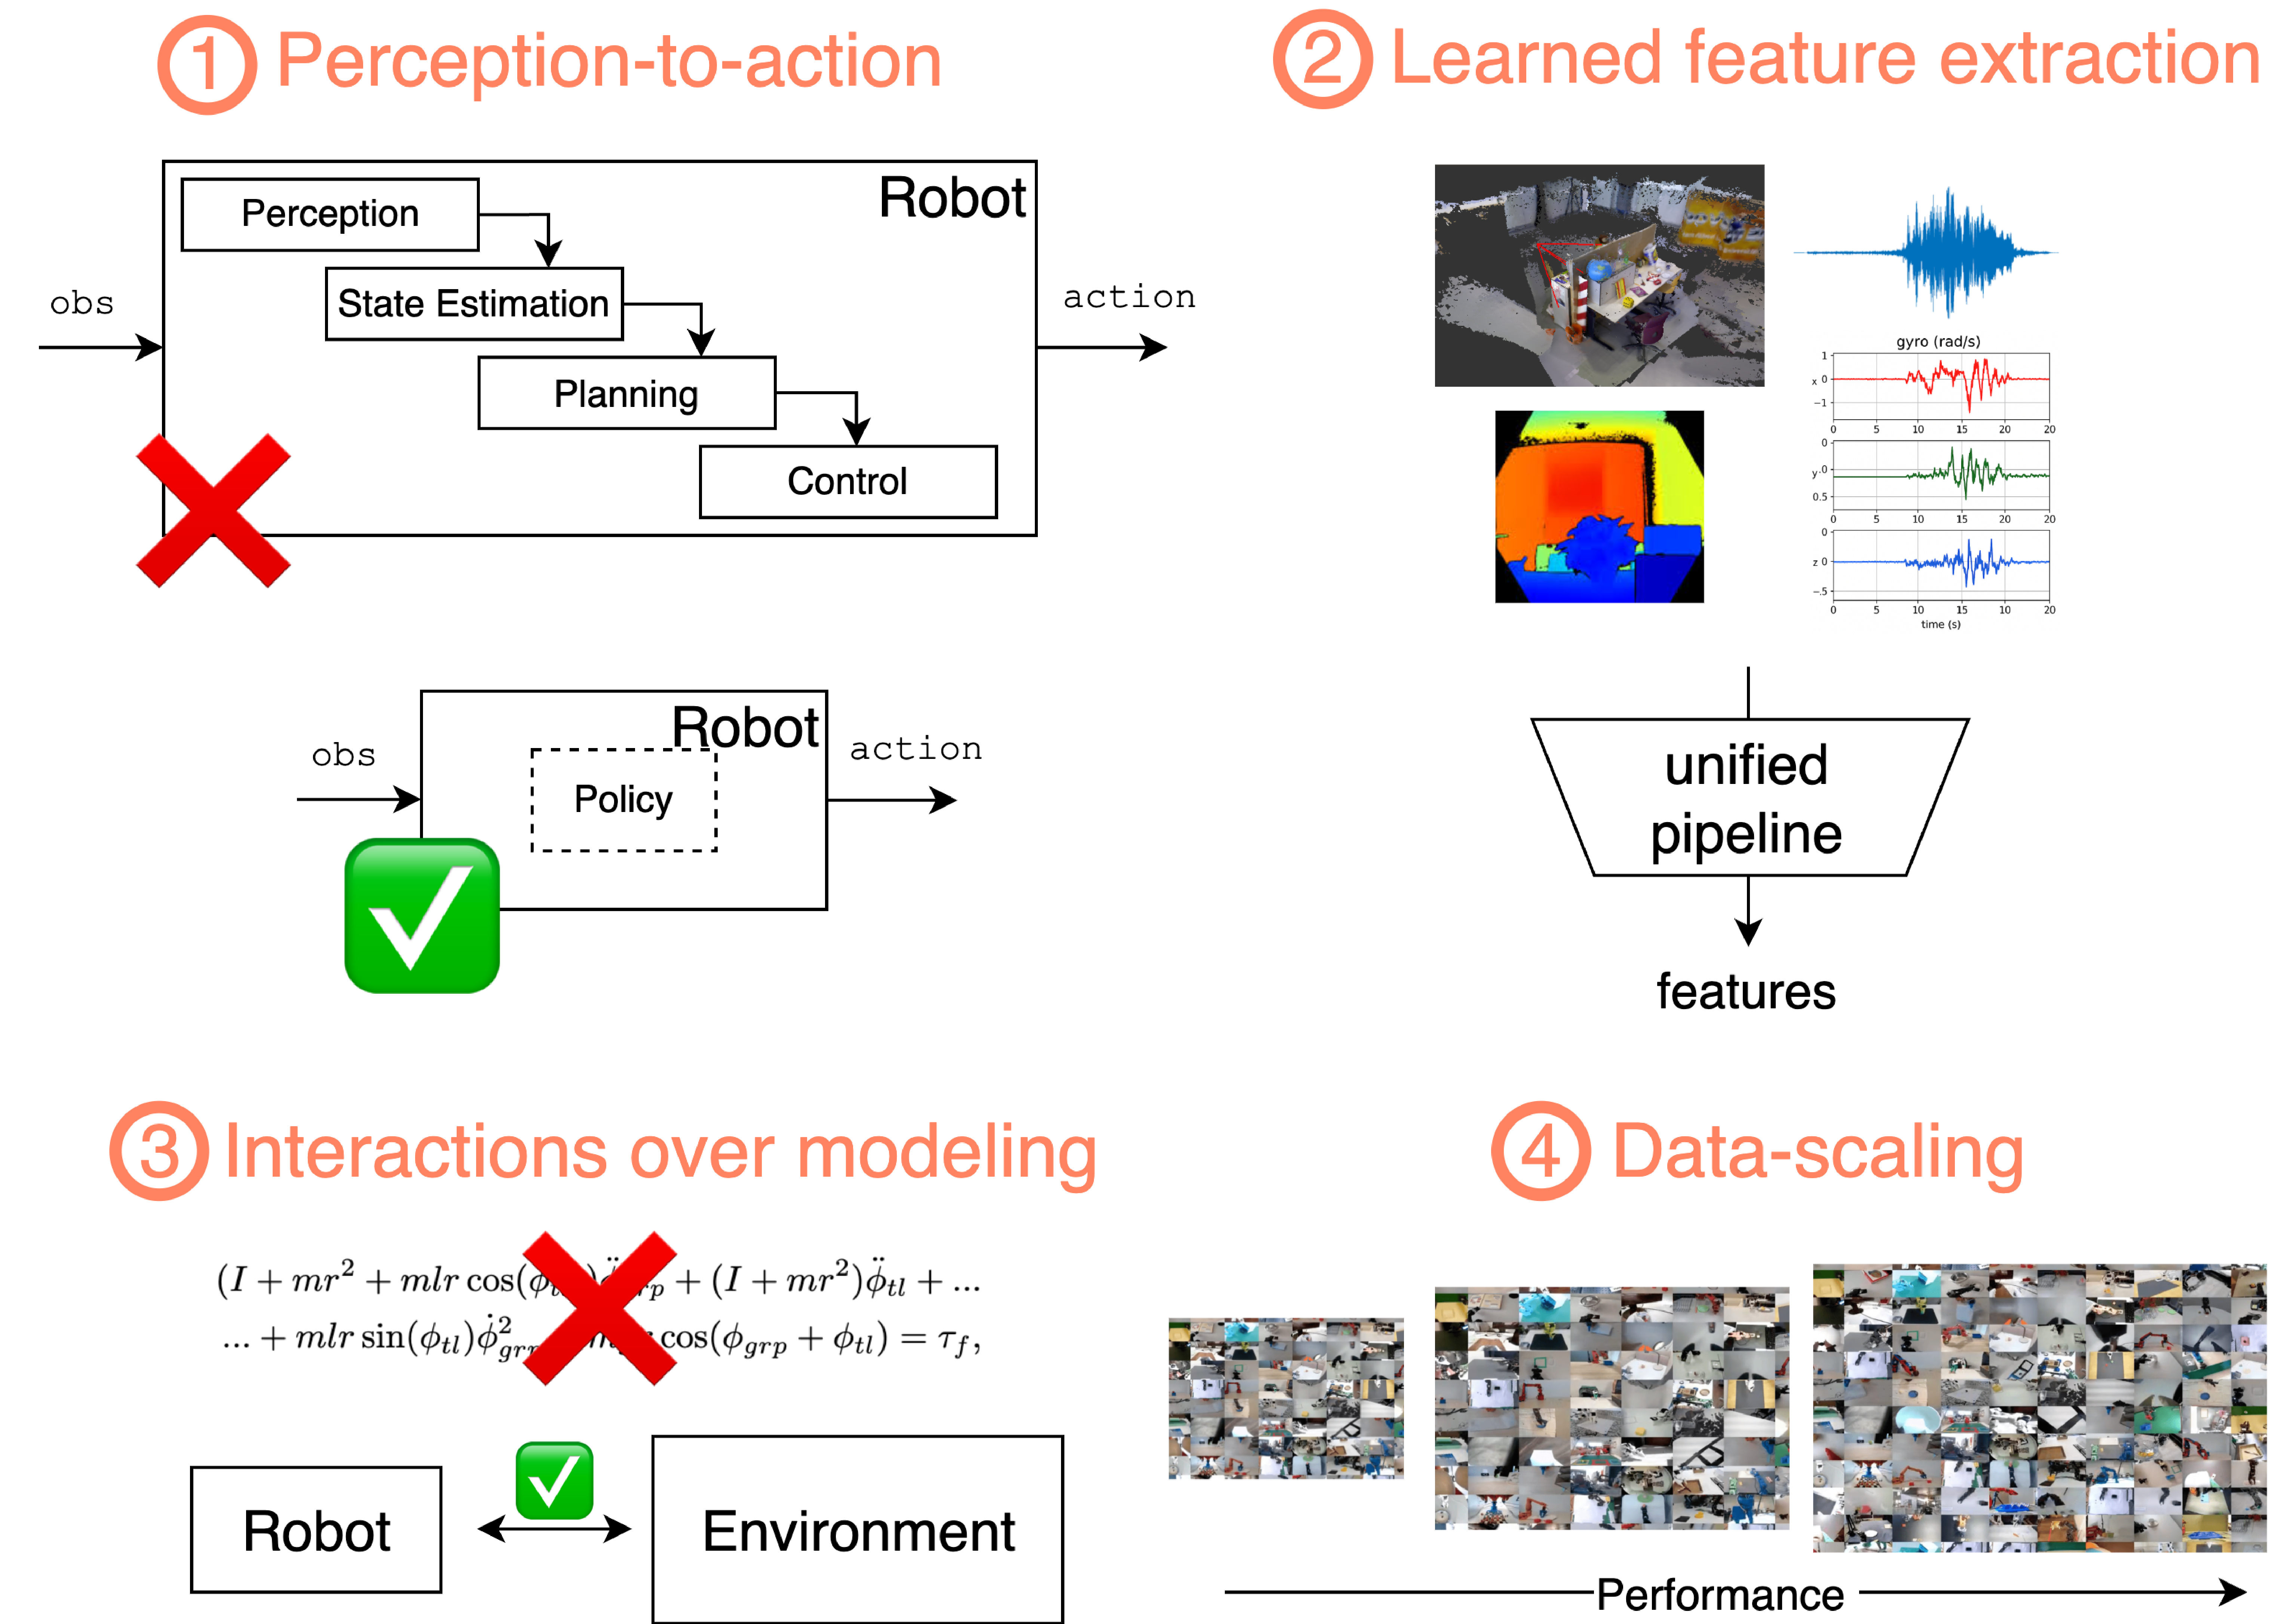
\includegraphics[width=\linewidth]{ch3/ch3-learning-benefits.png}
    \end{column}
    \begin{column}{0.42\textwidth}
      \begin{itemize}
        \item Learn a \highlight{single visuomotor policy} instead of stitching many modules together.
        \item Operate on raw, multimodal sensor streams.
        \item Optimize from experience without an explicit dynamics model.
      \end{itemize}
    \end{column}
  \end{columns}
\end{frame}

\begin{frame}{Robotics Tasks Naturally Fit the RL Loop}
  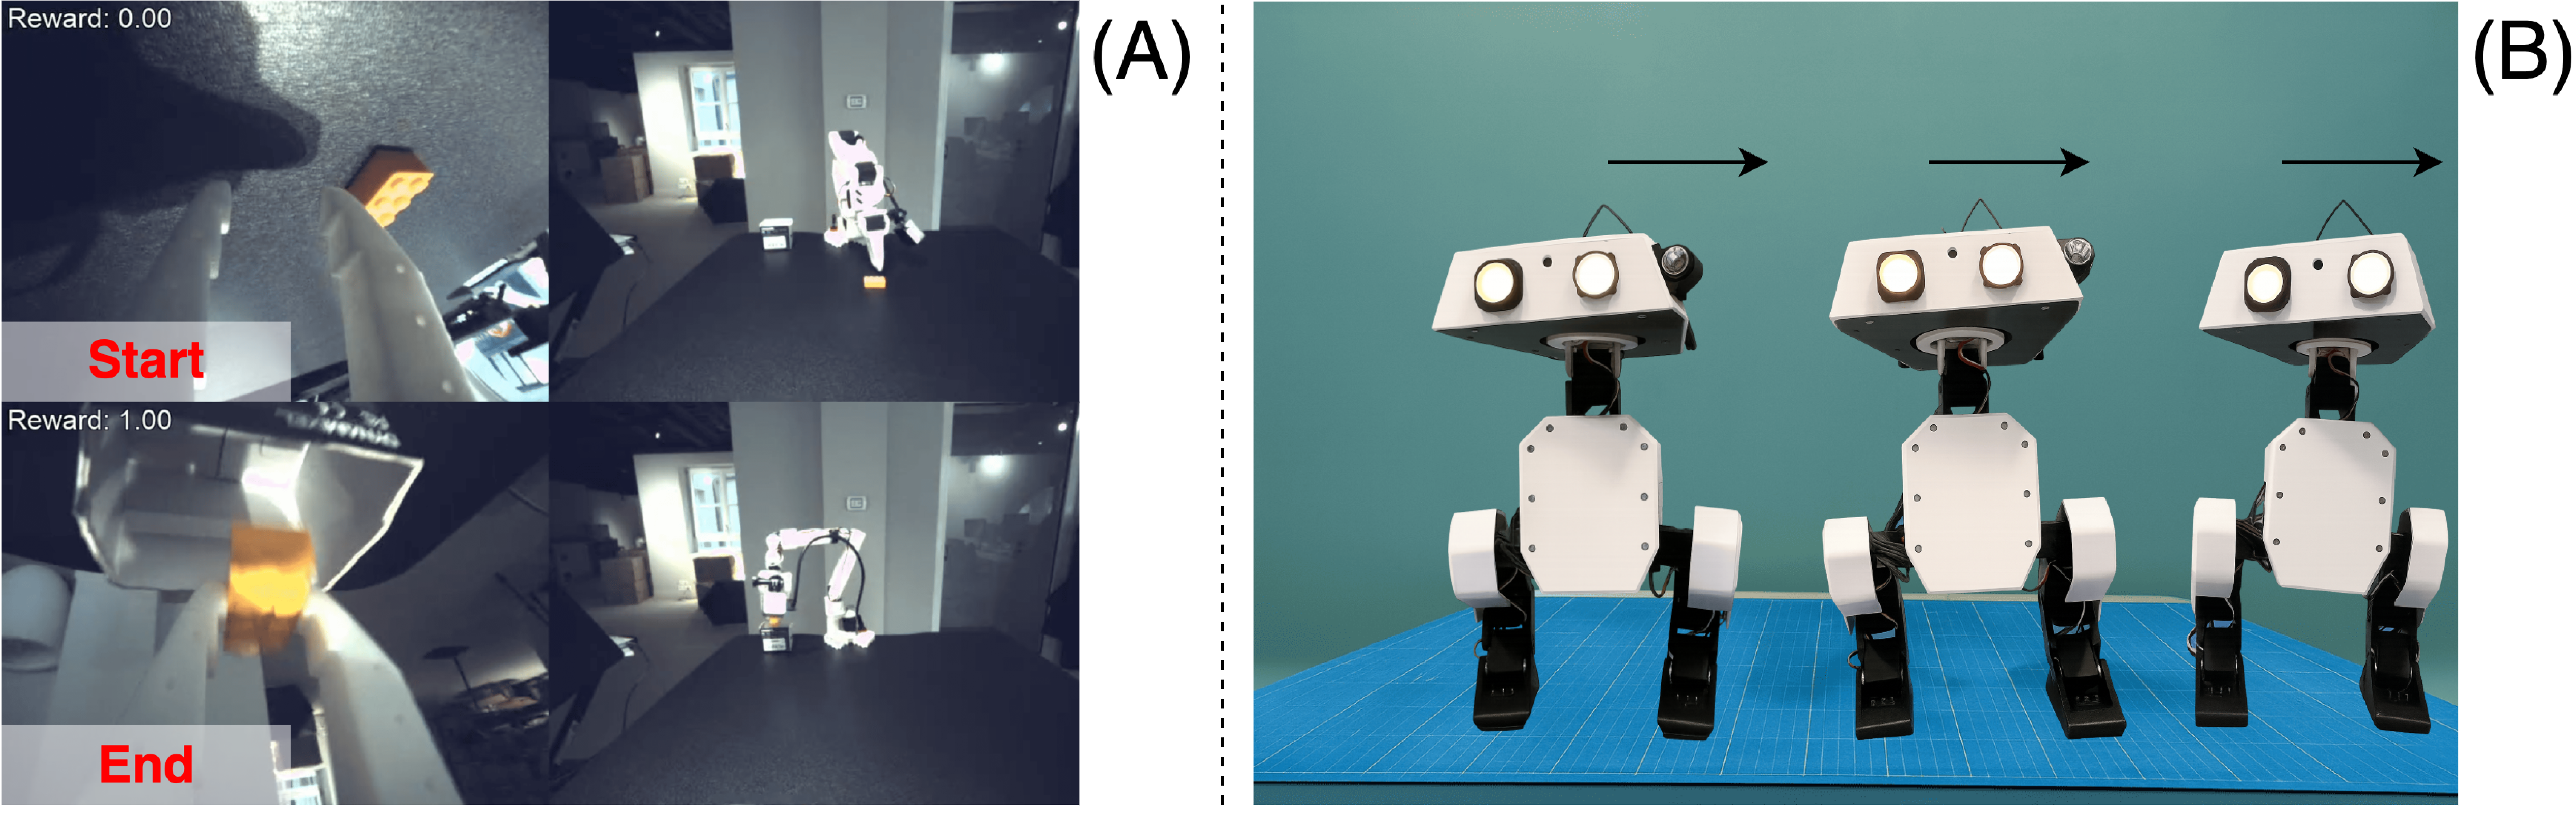
\includegraphics[width=\linewidth,height=0.68\textheight,keepaspectratio]{ch3/ch3-rl-examples.png}
  \begin{itemize}
    \item Manipulation and locomotion are both \highlight{sequential decision problems} with delayed consequences.
  \end{itemize}
\end{frame}

\begin{frame}{The Agent-Environment Interface}
  \begin{columns}[T,onlytextwidth]
    \begin{column}{0.42\textwidth}
      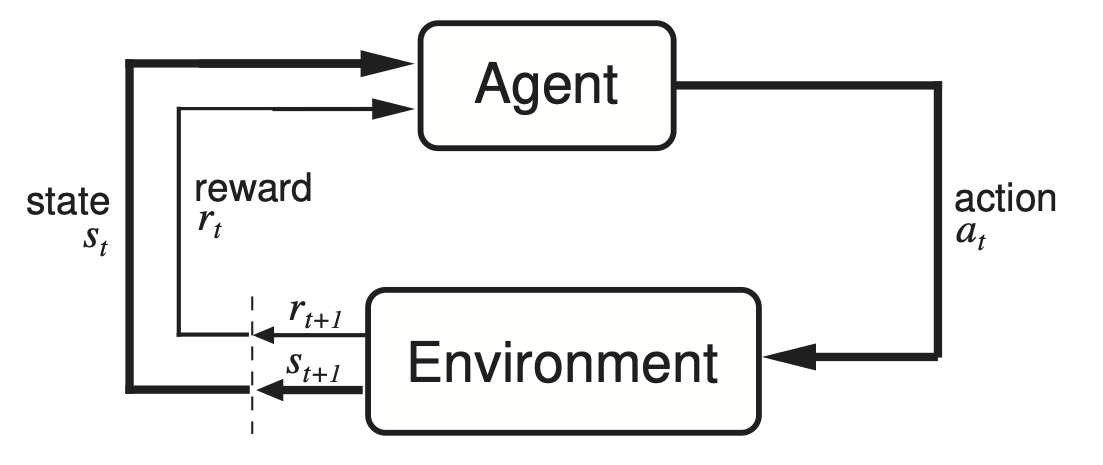
\includegraphics[width=\linewidth]{ch3/ch3-agent-env.png}
    \end{column}
    \begin{column}{0.54\textwidth}
      \begin{itemize}
        \item state \(s_t\): robot and environment information
        \item action \(a_t\): command applied to the system
        \item reward \(r_t\): scalar feedback about desirability
        \item dynamics: how the world evolves after each action
      \end{itemize}
    \end{column}
  \end{columns}

  \vspace{0.2cm}
  \statbox{Key abstraction}{RL turns control into repeated interaction: sense, act, observe consequences, improve.}
  \sources{\citep{suttonReinforcementLearningIntroduction2018}}
\end{frame}

\begin{frame}{What RL Optimizes}
  \[
  J(\pi)=\mathbb{E}\left[\sum_{t=0}^{T-1}\gamma^t r_t\right]
  \]

  \begin{itemize}
    \item The policy \(\pi\) should maximize long-horizon return, not just immediate reward.
    \item Value functions estimate how good states or state-action pairs are under a policy.
    \item In practice, these value estimates anchor many modern RL algorithms.
  \end{itemize}
\end{frame}

\begin{frame}{A Practical Algorithm Ladder}
  \begin{columns}[T,onlytextwidth]
    \begin{column}{0.38\textwidth}
      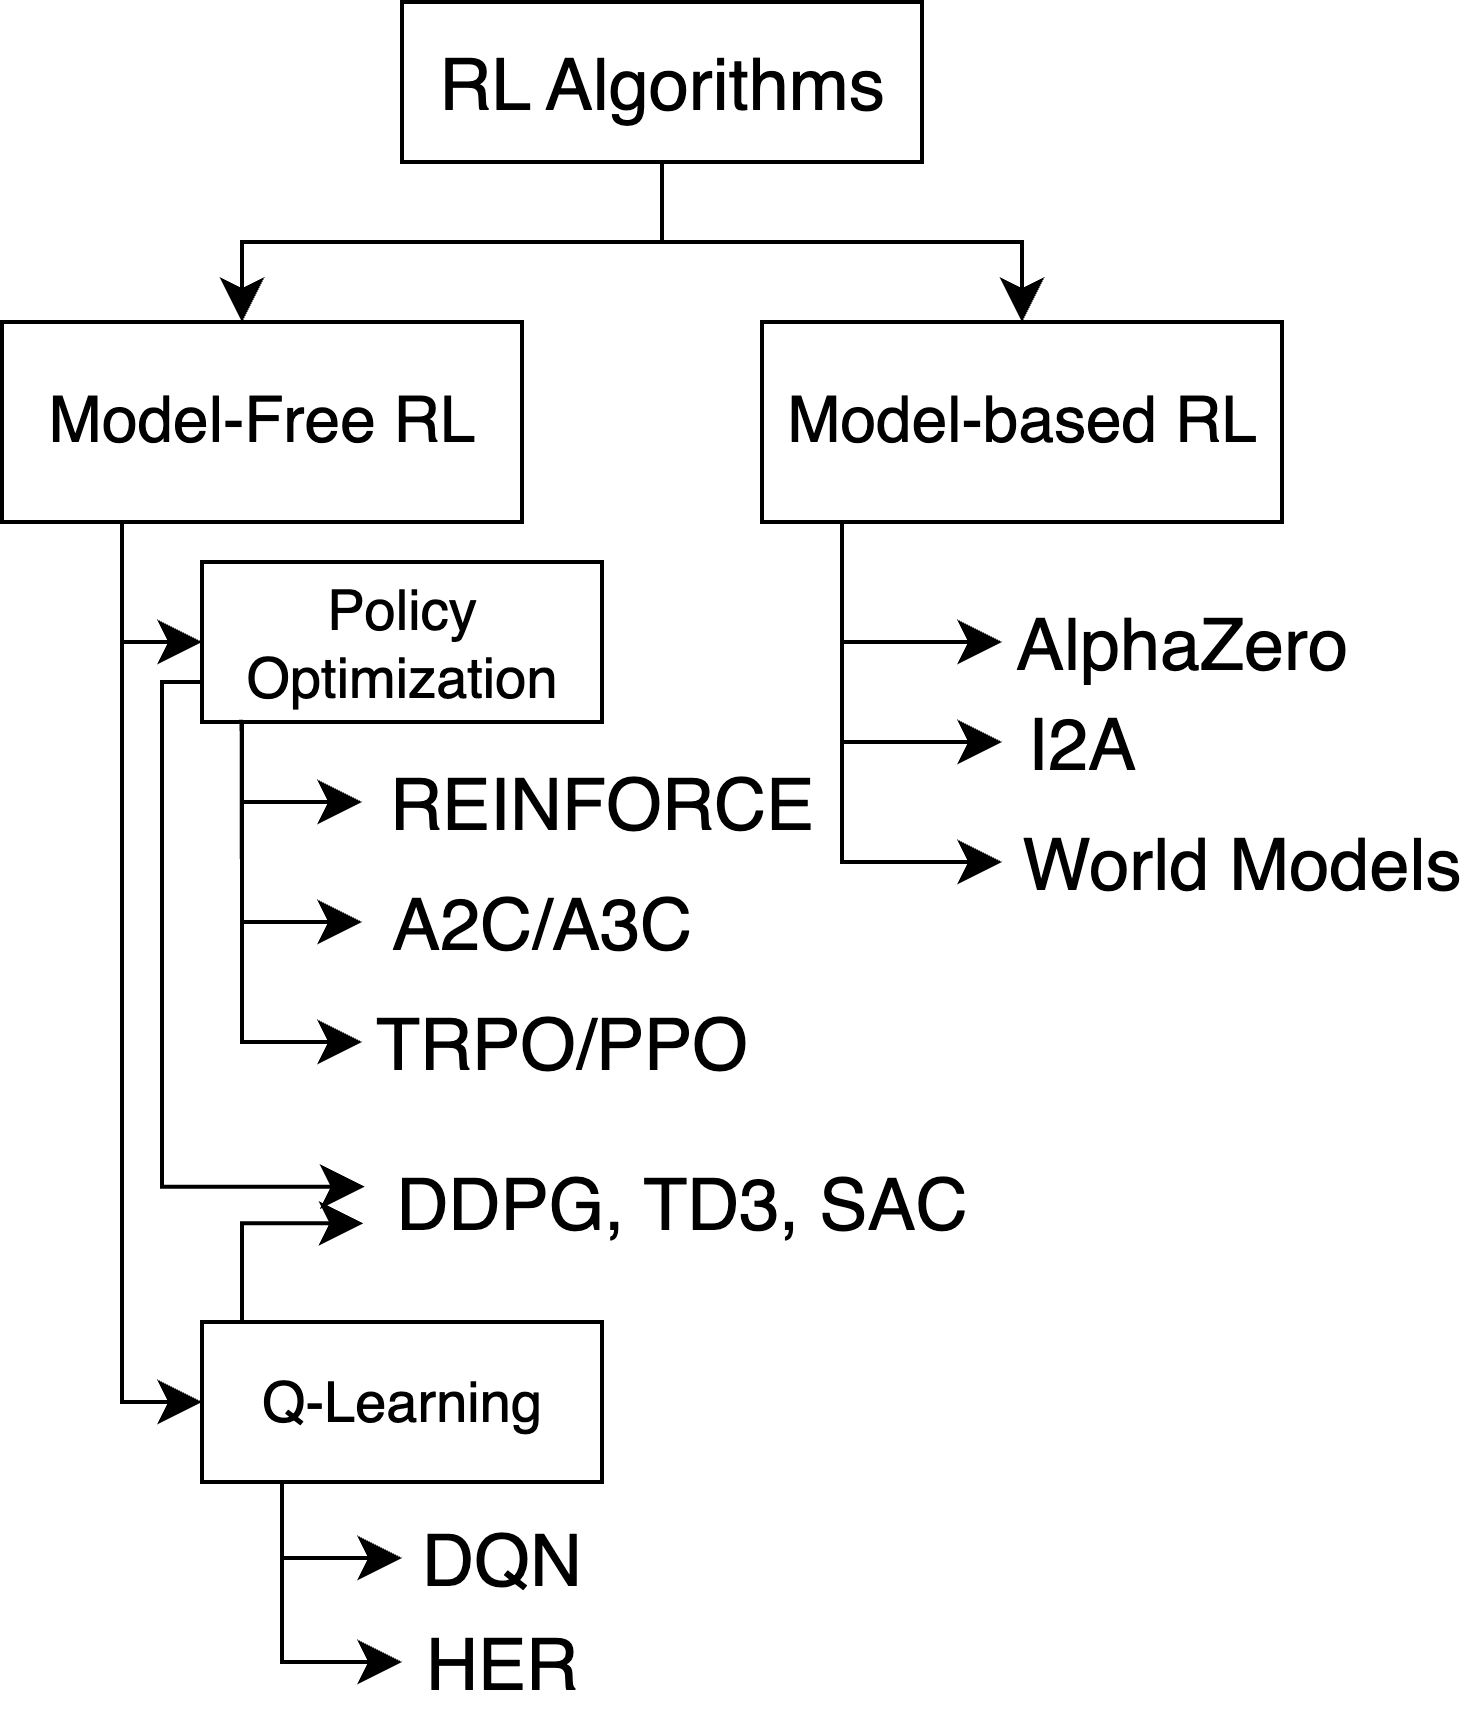
\includegraphics[width=\linewidth]{ch3/ch3-rl-algorithms-atlas.png}
    \end{column}
    \begin{column}{0.58\textwidth}
      \begin{itemize}
        \item Value iteration and Q-learning motivate data reuse.
        \item DQN scales value learning to large observation spaces.
        \item DDPG handles continuous control with an explicit actor.
        \item SAC adds entropy regularization for robustness and exploration.
      \end{itemize}
    \end{column}
  \end{columns}
  \sources{\citep{mnihPlayingAtariDeep2013,pmlr-v32-silver14,lillicrapContinuousControlDeep2019a,haarnojaSoftActorCriticOffPolicy2018}}
\end{frame}

\begin{frame}{Why Real-World RL Is Hard}
  \begin{itemize}
    \item Early exploration is often \highlight{unsafe and erratic} on hardware.
    \item Real robots are slow to reset, expensive to supervise, and costly to wear out.
    \item Sample inefficiency is especially painful when every transition must be collected physically.
    \item Dense rewards are hard to write for contact-rich, visually grounded tasks.
  \end{itemize}

  \vspace{0.25cm}
  \statbox{Main tension}{RL is conceptually elegant for robotics, but naive online training is often impractical on the real world.}
\end{frame}

\begin{frame}{Simulation Helps, Then Hurts}
  \begin{columns}[T,onlytextwidth]
    \begin{column}{0.52\textwidth}
      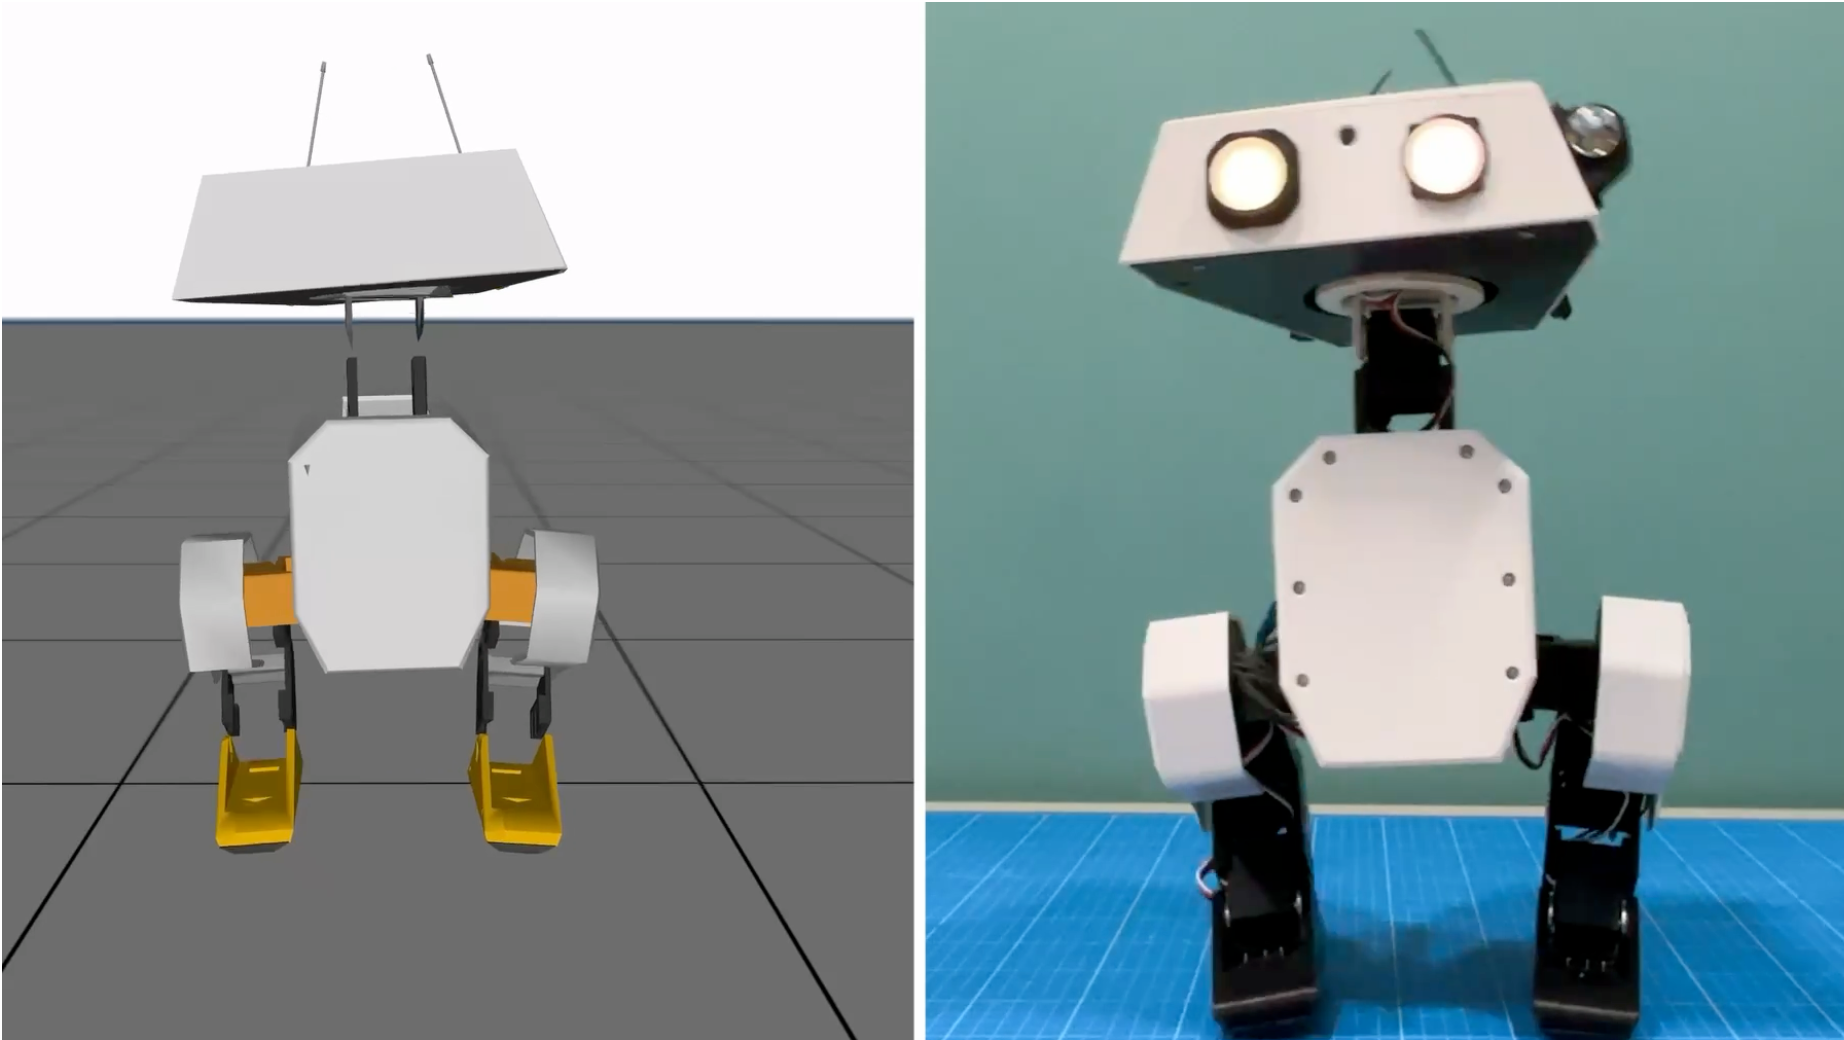
\includegraphics[width=\linewidth]{ch3/ch3-duck-sim-vs-real.png}
    \end{column}
    \begin{column}{0.44\textwidth}
      \begin{itemize}
        \item Simulation removes physical risk and speeds up training.
        \item But transfer is limited by the \highlight{reality gap}: modeling assumptions do not perfectly match hardware.
      \end{itemize}
    \end{column}
  \end{columns}
\end{frame}

\begin{frame}{Domain Randomization Is Useful, but Manual}
  \begin{columns}[T,onlytextwidth]
    \begin{column}{0.58\textwidth}
      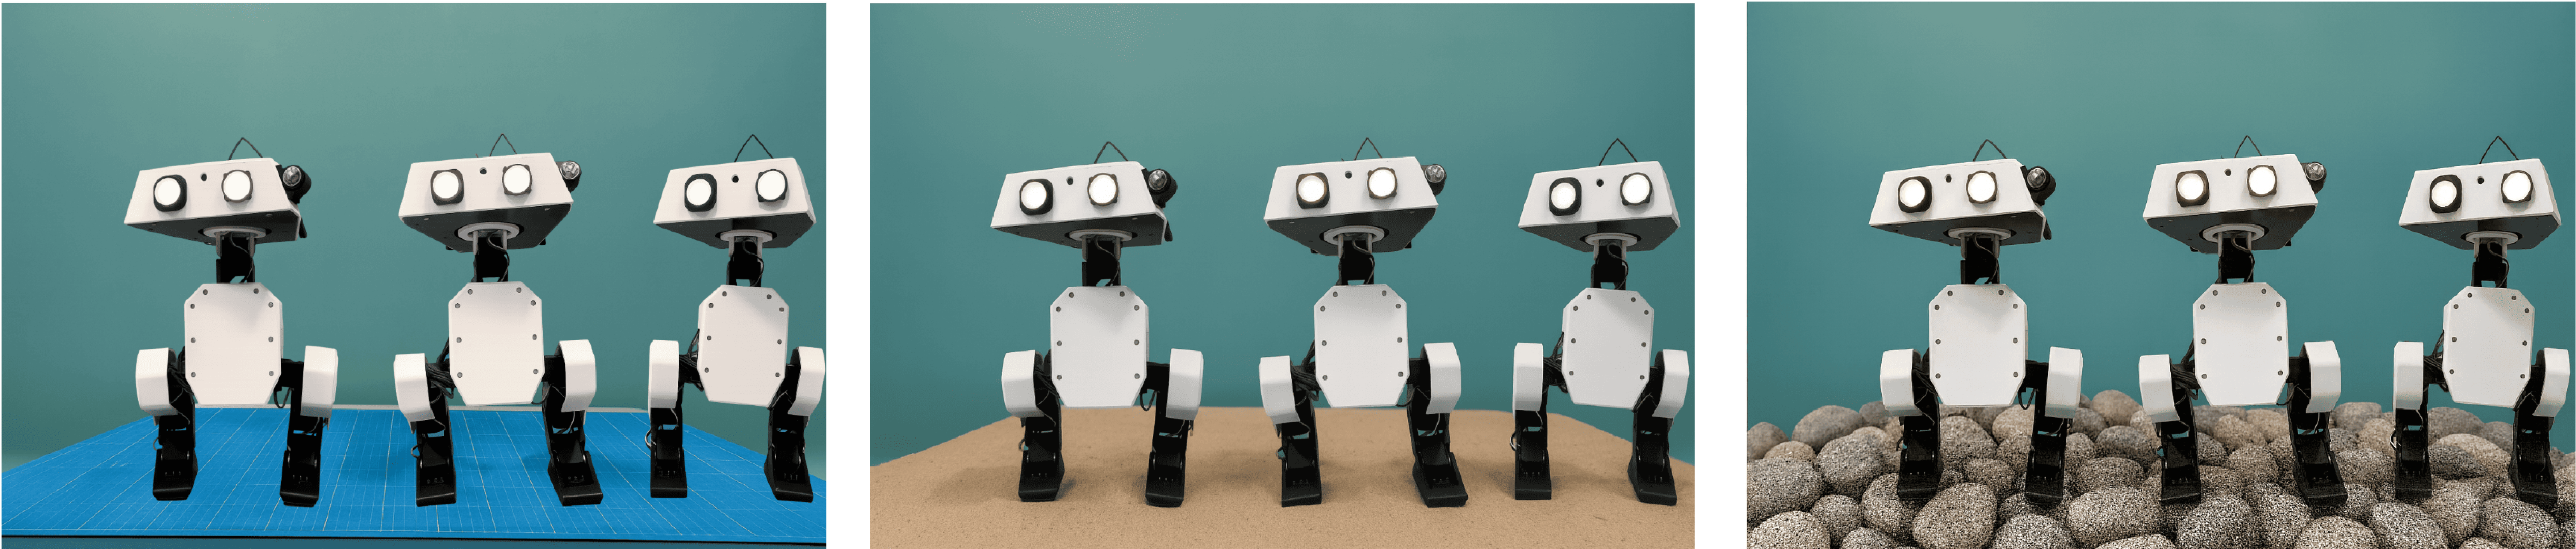
\includegraphics[width=\linewidth]{ch3/ch3-many-ducks.png}
    \end{column}
    \begin{column}{0.38\textwidth}
      \begin{itemize}
        \item Randomize terrain, friction, mass, lighting, or other dynamics.
        \item Goal: learn policies robust to a \highlight{distribution of worlds}.
        \item Problem: choosing what to randomize and how much is itself brittle.
      \end{itemize}
    \end{column}
  \end{columns}
  \sources{\citep{tobinDomainRandomizationTransferring2017,akkayaSolvingRubiksCube2019,tiboniDomainRandomizationEntropy2024}}
\end{frame}

\begin{frame}{Off-Policy RL Makes Data Reusable}
  \begin{itemize}
    \item Replay buffers let the agent train on past transitions multiple times.
    \item That is why algorithms like SAC are attractive for robotics: they are \highlight{more sample efficient}.
    \item Prior demonstrations can also be injected into the same training pipeline.
    \item This creates a bridge from pure RL toward offline-to-online robot learning.
  \end{itemize}
\end{frame}

\begin{frame}{From Prior Data to SERL}
  \begin{itemize}
    \item RLPD mixes offline demonstrations with online data instead of learning from scratch.
    \item SERL adds \highlight{reward classifiers} to avoid hand-writing dense rewards from images.
    \item SERL also uses forward and backward controllers so the robot can learn both task completion and reset behavior.
  \end{itemize}

  \vspace{0.2cm}
  \statbox{Why this matters}{The pipeline becomes safer, more data-driven, and materially more realistic for real hardware training.}
\end{frame}

\begin{frame}{HIL-SERL Adds Targeted Human Corrections}
  \begin{columns}[T,onlytextwidth]
    \begin{column}{0.56\textwidth}
      \includegraphics[width=\linewidth]{ch3/ch3-hil-serl-examples.png}
    \end{column}
    \begin{column}{0.4\textwidth}
      \begin{itemize}
        \item Expert trajectories seed the policy.
        \item Human interventions correct failure modes online.
        \item Intervention data is replayed aggressively, giving the agent strong supervision where it matters most.
      \end{itemize}
    \end{column}
  \end{columns}
  \sources{\citep{luoPreciseDexterousRobotic2024}}
\end{frame}

\begin{frame}{HIL-SERL in \lerobot}
  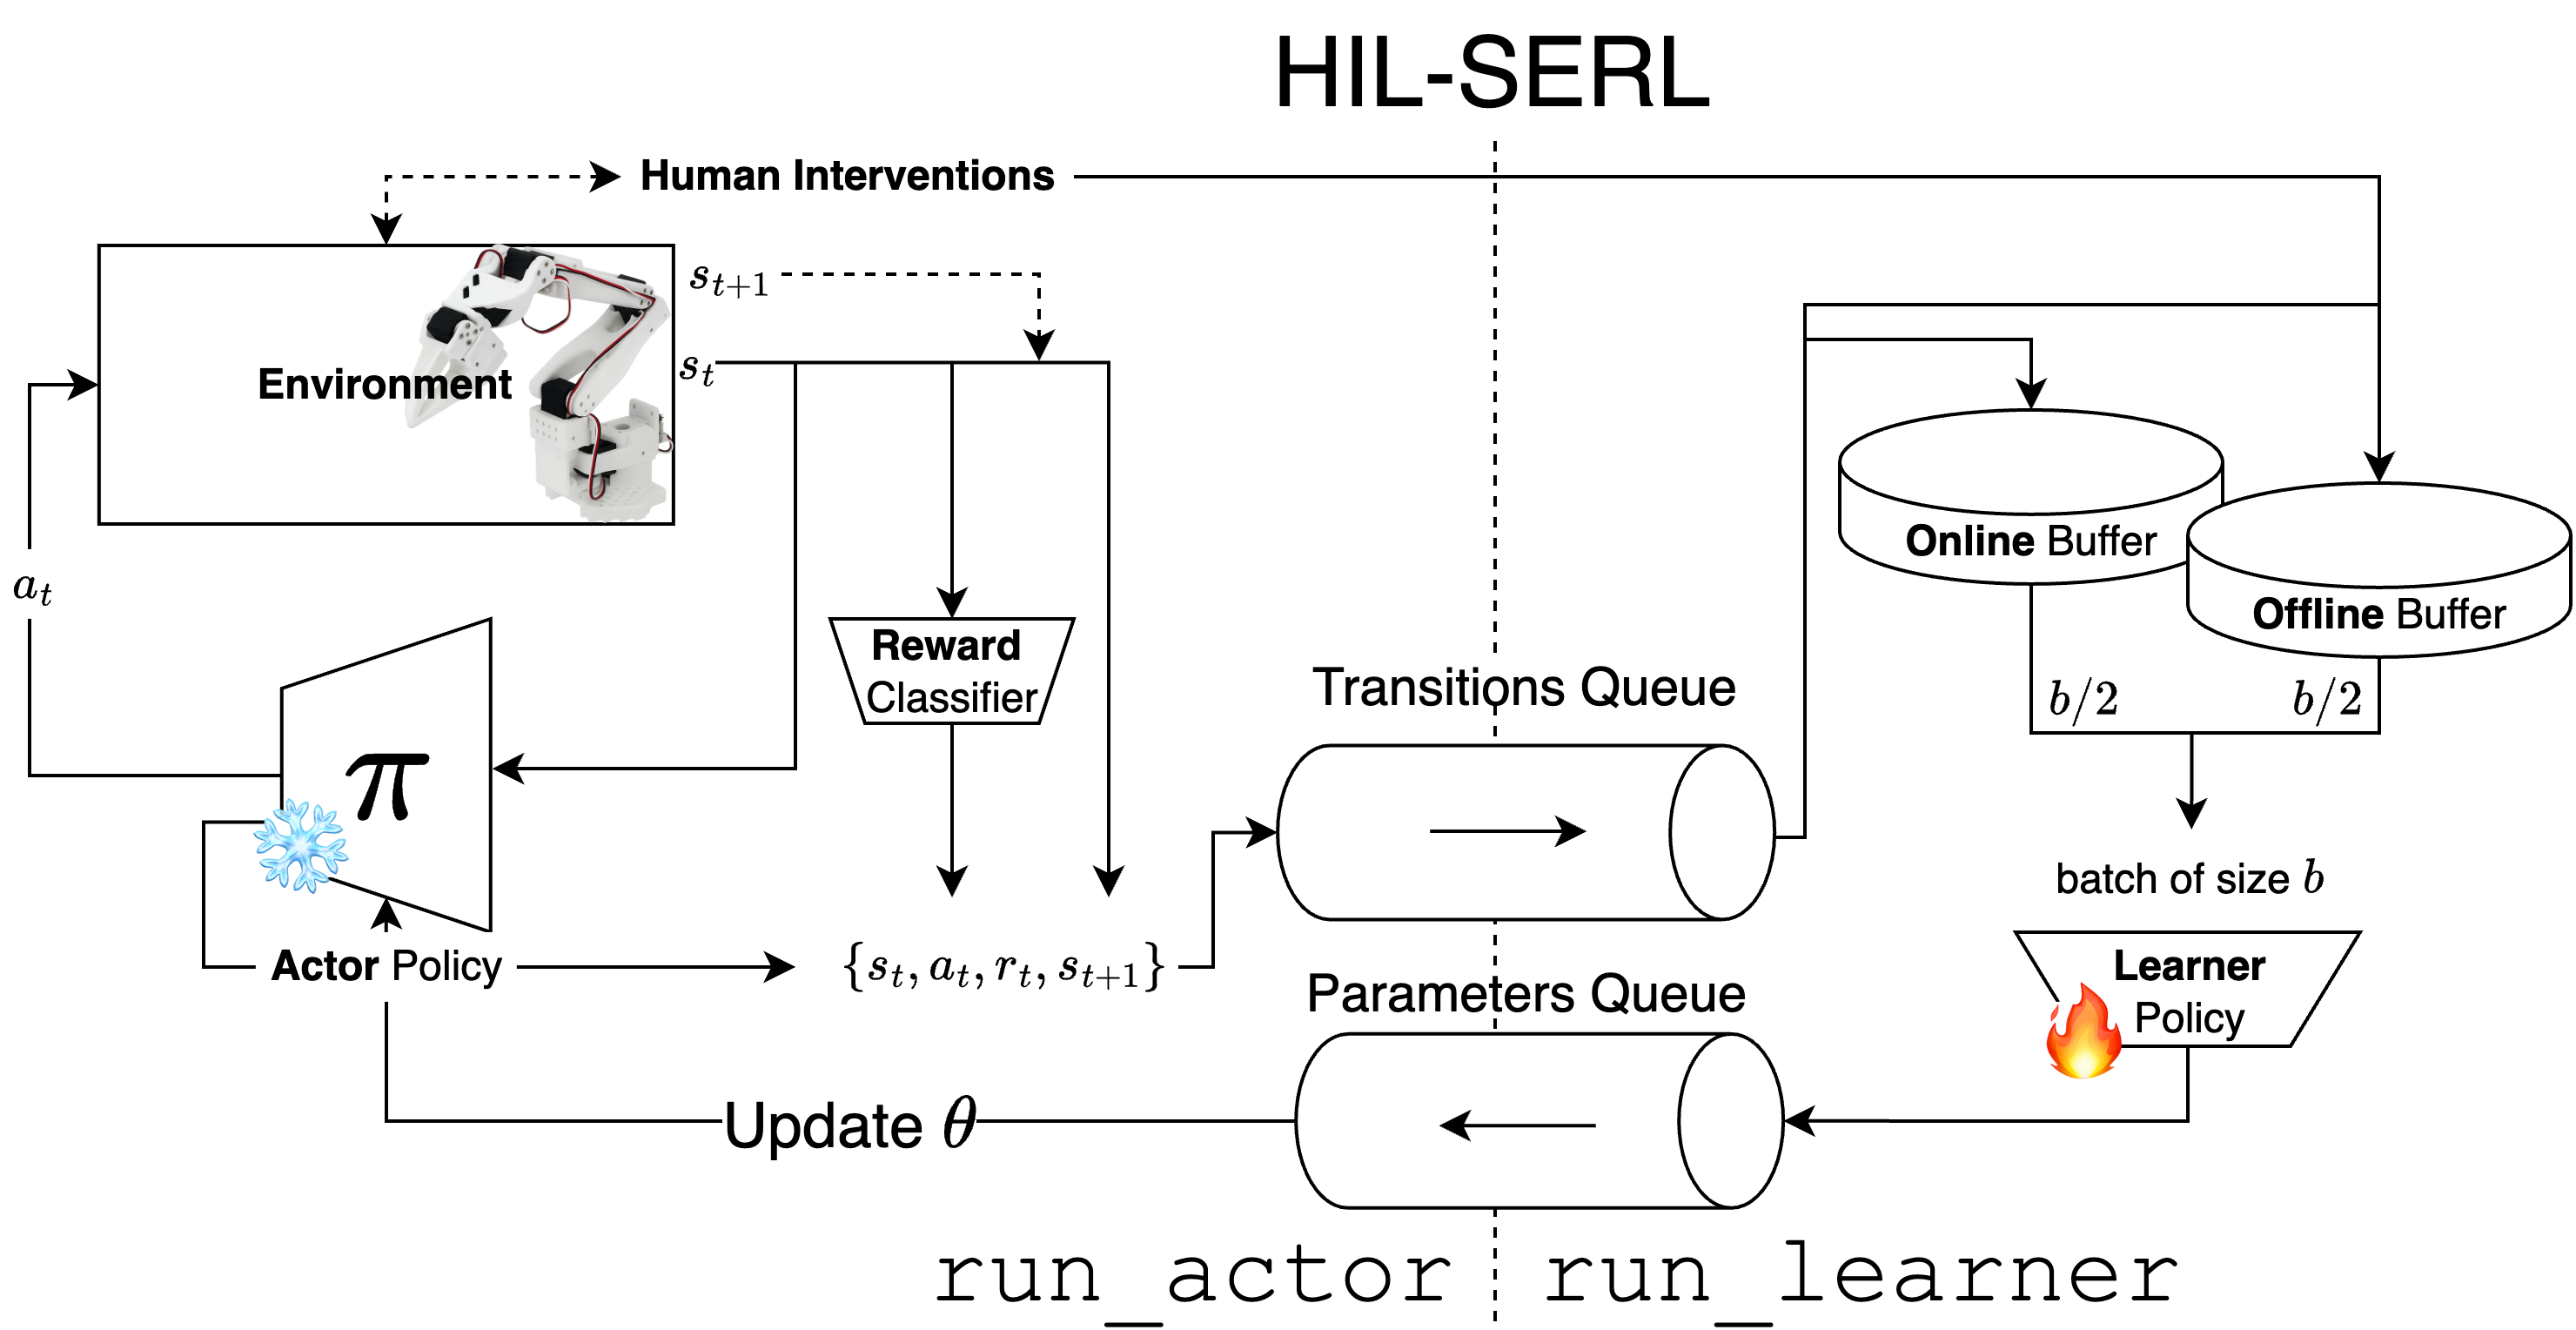
\includegraphics[width=\linewidth,height=0.55\textheight,keepaspectratio]{ch3/ch3-hil-serl-architecture.png}

  \begin{itemize}
    \item \textbf{Actor}: interacts with the robot, computes rewards with the classifier, sends transitions.
    \item \textbf{Learner}: samples offline and online buffers, updates parameters, sends weights back.
    \item The same split can run locally or across machines.
  \end{itemize}
\end{frame}

\begin{frame}{Practical Use in \lerobot}
  \begin{block}{Core pieces}
    Reward classifier, actor, learner, and a final orchestration script.
  \end{block}

  \begin{itemize}
    \item Reference snippets:
    \item \texttt{snippets/ch3/01\_reward\_classifier.py}
    \item \texttt{snippets/ch3/02\_actor.py}
    \item \texttt{snippets/ch3/03\_learner.py}
    \item \texttt{snippets/ch3/04\_hil\_serl.py}
  \end{itemize}
\end{frame}

\begin{frame}{Why BC Still Becomes the Next Step}
  \begin{itemize}
    \item Some tasks remain hard to simulate faithfully.
    \item Some tasks remain hard to reward robustly.
    \item Learning from demonstrations avoids both burdens, even if it gives up the possibility of strongly surpassing the demonstrator.
  \end{itemize}

  \vspace{0.25cm}
  \statbox{Chapter takeaway}{RL gives a principled framework for robot control, but real-world usability depends on prior data, reward learning, and human guidance. Those pressures motivate imitation learning.}
\end{frame}

\begin{frame}[allowframebreaks]{Selected References}
\scriptsize
\nocite{ballEfficientOnlineReinforcement2023}
\bibliography{../shared/references}
\end{frame}

\end{document}
